\subsection{Tool comparison on synthetic data}\label{app:synthetic}

\begin{figure*}[t]
  \centering
  \subfloat[$d{=}1\%$, exact matches]{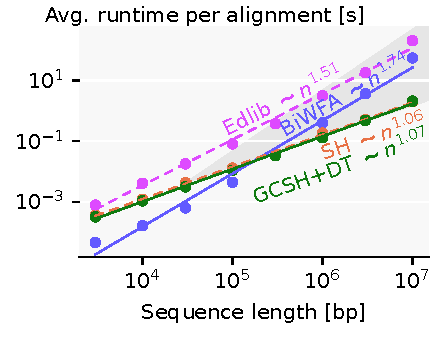
\includegraphics[scale=0.75]{plots/tools_e0.01.labels.pdf}
  \label{fig:tools-1}}
  \hfill
  \subfloat[$d{=}4\%$, exact matches]{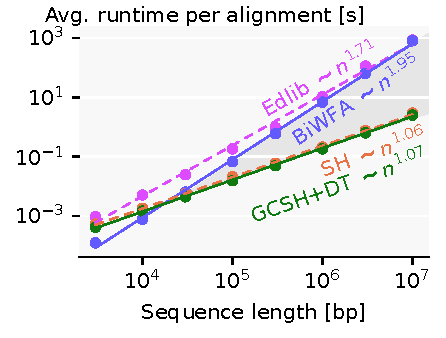
\includegraphics[scale=0.75]{plots/tools_e0.05.labels.pdf}
  \label{fig:tools-5}}
  \hfill
  \subfloat[$d{=}8\%$, inexact matches]{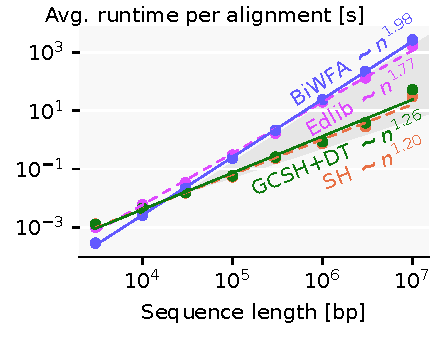
\includegraphics[scale=0.75]{plots/tools_e0.10.labels.pdf}
  \label{fig:tools-10}}
  \hfill
  \subfloat[$d{=}12\%$, inexact matches]{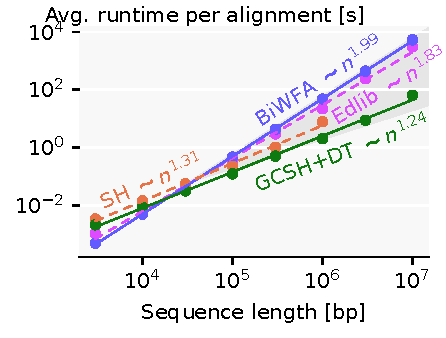
\includegraphics[scale=0.75]{plots/tools_e0.15.labels.pdf}
  \label{fig:tools-15}}
  \caption[Runtime scaling with sequence length on synthetic data]{\textbf{Runtime scaling with sequence length on synthetic data.}
  Log-log plots comparing our simplest heuristic~(\SH) and our most accurate
  heuristic~(\GCH, with DT) with \edlib and \wfa. The slopes of the bottom (top)
  of the dark-grey cones correspond to linear (quadratic) growth. The seed
  length is~$k{=}15$ and for~$d{\geq}8\%$ the heuristics use inexact
  matches~($r{=}2$). Averages are over total~$N{=}10^7\bp$. The missing data
  points for~\SH at~$d{=}12\%$ are due to exceeding the $\qty{32}{GiB}$ memory
  limit.}
  \label{fig:tools}
\end{figure*}

In~\cref{fig:tools} we compare our \A heuristics with \edlib and \wfa in terms
of runtime scaling with sequence length $n$ and divergence $d$.
